\section{Introduction}
\label{sec:intro}

 
Engineering is a challenging discipline to study, and doubly so for students from groups that are underrepresented in engineering who deal with discrimination, bias, microaggressions, and other forms of “othering” during their careers. These groups include racial and ethnic minorities (e.g., McGee, 2011), women (e.g., Moss-Racusin, 2012), LGBTQIA-identifying students (e.g., Cech, 2011) and first-generation college students (e.g., Pascarella, 2004, Carrigan, et al., 2019). These challenges can be compounded when multiple identities come into play (e.g., Williams, 2014). Despite significant funding and attention paid to diversity in engineering, the percentage of B.S. degrees awarded to women in 2017 was just 21.3\%.  This is even more distressing because this was a 10-year high (ASEE 2017). 

 
Although the experiences of minority populations have been studied for some time now, this is a very challenging field to make progress on. It can be particularly difficult to effectively measure the impact of problems, and of solutions, on students. This is work that typically must be very specific and focused. For example, take the question of bias against women. It can be difficult to prove that bias exists, and is caused by gender, but in the case of resume assessments, a clever way to measure bias is to vary the name (and nothing else) in a resume. Using this approach, multiple studies have demonstrated bias in assessment of resumes based on presumed gender. In one recent double-blind study, 127 faculty in biology and physics each reviewed an undergraduate resume with a randomly assigned female or male name for a fictional lab manager position (Moss-Racusin, 2012). Men were rated as being more competent, hireable, and worthy of mentoring and higher pay than women. Reviewer gender, seniority, field, and age had no effect on outcome. An earlier psychology study of 238 faculty who received four gender-randomized resumes showed similar outcomes (Steinpreis, 1999). Still, the impact of those biases is hard to measure, especially since they are often small and may take years to add up. However, the impact of small differences in evaluation of female candidates of 1-5\% (a purported degree to which gender bias affects performance ratings (Barrett, 1993)) can be used to simulate how discrimination will impact gender distributions over time in an organization (Martell, 1996), as well as productivity (Cole 1991). In simulation, such differences accumulate, leading to approximately a 2:1 difference in measures of success between men and women at the most senior levels (Cole, 1991; Martell, 1996). At the end of decades of work, we have a model (though no field test) of impact, and still no solution -- no field-tested technique for reducing this bias, or its impact. And this body of work was focused almost entirely on resume assessment of women, just a small drop in the bucket of the bigger picture for minority students attempting to succeed in their fields. How, then, can we expect to solve these problems? \paula{comment}
 
We argue that what is needed is a far more comprehensive approach to data collection. In the era of big data, there is no excuse for small studies, in which a study of 238 faculty, focused on just one issue, is considered impressive. What is needed is a comprehensive change in the way that we collect and assess the college student experience, in particular, one that tackles our understanding of bias in a new way. And the technological innovations needed to make this possible are here -- we have access to devices that can passively capture many of the activities that students engage in; and technical approaches that can actively capture the remainder of the information we need to know. This is an exciting era for data collection and analysis and one in which it becomes possible to study issues such as discrimination and bias, at scale and in real-time, and truly understand their impact. This important information will help support the design of effective interventions, policy, and decision making to improve the experiences of not just diverse students in engineering, but all students in engineering. 
 
To date, we have done pilot work, at the scale of 350 students across two years (including 50 students who participated both years). While we are still collecting year 2 data, our first year of data analysis  shows that this approach is a feasible technique. Participants reported almost 450 separate instances of discrimination and numerous other major and minor life events that impacted their daily school experience. Our proposal is to scale up this study to four years, so that we can truly understand the impact of many separate facets of engineering on students’ experiences and success. We focus specifically on underrepresented groups in engineering, which we call UREs. This includes women, underrepresented minorities, first-generation college students, and LGBTQ students. Our pilot data show that all of these groups are at risk for discrimination and other obstacles that may impact retention. Further, we argue that an intersectional approach is critical to understanding the challenges these groups face. Thus, we consider discrimination, harassment, and other challenges together with a range of identities in a single holistic study.  
 

\subsection{Intellectual Merit}
\label{sec:questions}

We  propose to test a model of the student experience (shown in Figure~\ref{fig:model} ) that we believe helps to capture the differential stressors experienced by women and minorities in a way that can ultimately be quantified and operationalized. We anticipate detecting meaningful changes in behavior associated with such distress. Our focus in this work is thus on quantifying such changes, and how interventions and micro-climates impact them, based on objective unobtrusive measures of phone and wearable data. Our work will make it possible to document, for the first time, \textit{what behaviors change and in what ways} following discrimination.  

\begin{figure}
    \centering
    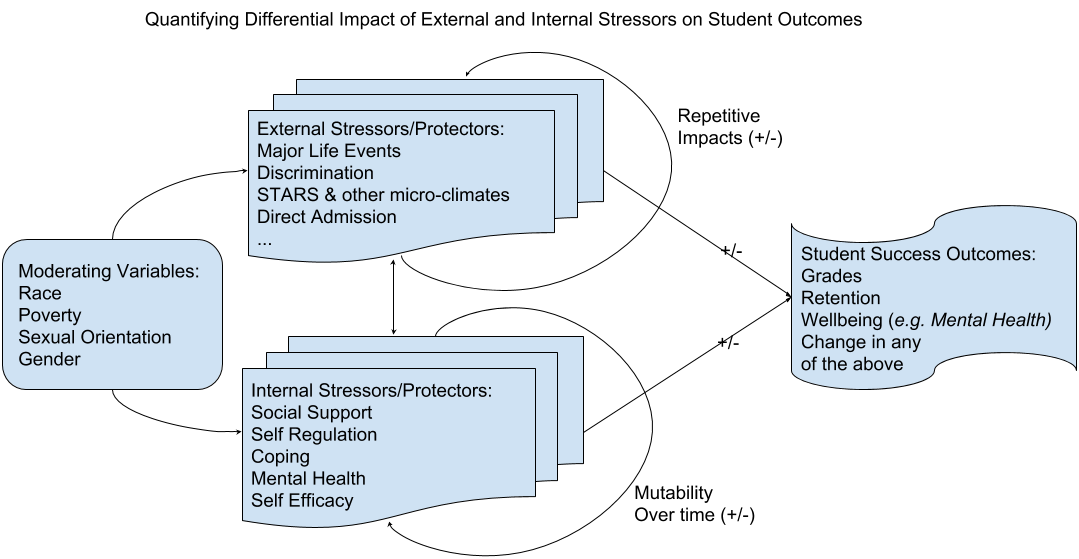
\includegraphics[width=12cm]{img/model2.png}
    \caption{Relating behavioral variables and outcomes}
    \label{fig:model}
\end{figure}

Our goal is to develop a holistic understanding of the impacts of personal background (as it plays out during the educational experience) and climate on the participation and retention of UREs over their college career. It is important to consider both -- we are failing students if we situate problems entirely in the individual instead of considering system and climate issues, but the impact of climate cannot be understood without considering individual differences and historical and current experiences. We propose to follow a cohort of students throughout four years of their engineering education. In addition to capturing descriptive data about the student experience, we will compare the impact of the existing microclimate programs within the College of Engineering, specifically students who experience no microclimate, students in SEEEDS and students in the NSF-funded STARS program.  This will help us to develop a deeper understanding of how various programs and interventions impact the student experience and generate recommendations for future intervention development.
%Passive sensing through mobile phones and wearables is a promising approach to capturing behaviors that are indicative of mental states. This approach would allow us to investigate the understudied topic of short-term behavior changes associated with discrimination. Without reporting specifics, the little existing work suggests psychological distress shortly follows discrimination. 
To quantify difference, we ask: %\yasaman{Analysis of the global behavior patterns and discrimination is similar to the analysis in paper tracking depression dynamics by Campbell’s group in UbiComp’18 that looked at PHQ8 and behavior patterns.}

\begin{enumerate}[start=1,label={\bfseries RQ\arabic*}, leftmargin=1cm]
    \item \label{itm:rq-long-outcome} What are the differences in mental health (\eg anxiety, depression, or loneliness) between people who have reported discrimination and people who have not?
    \item \label{itm:rq-long-behavior} Do these differences also exist at the level of \textit{global} behavior patterns (\ie behaviors aggregated for the duration of the study) as captured by phone and wearable sensors?
    \item \label{itm:rq-short-outcome} What are the changes in self-reported daily affect following reports of discrimination? %\yasaman{to be later considered: differences in daily stress health behavior}
    \item \label{itm:rq-short-behavior} Are there changes at the level of behavior patterns captured by phone and wearable sensors?
\end{enumerate}

\noindent Turning to assessing micro climates, we ask:

\begin{enumerate}[start=3,label={\bfseries RQ\arabic*}, leftmargin=1cm]
   \item \label{itm:intervention1} How does an intervention such as STARS change the micro-climate experienced by students xxx 
    % \item \label{itm:rq-short-within} What are the changes in self-reported daily affect, stress, and health behavior, as well as behavior patterns captured by phone and wearable devices that are associated with incidents of discrimination?
    % \item \label{itm:rq-short-change} Should there be any changes:
    % \begin{itemize}
    %     \item How strong are they?
    %     \item What are the temporal dynamics (\eg onset and duration) of the changes?
    %     \item Are there any inter-relations between the various changes?
    % \end{itemize}
\end{enumerate}

\noindent
These research questions are by no means the only things that can be asked of our data set, and given the cost and size of the study this is intentional -- it is our plan to use this data set to foster a wide range of impactful research. However, they are our focus in this proposal for two important reasons:
(1) We believe that they can directly support policy makers at our university and beyond in determining appropriate considerations when trying to meet the needs of the populations we are studying. 
(2) The answers to these questions will directly feed into our own goal of creating and deploying interventions that help to create protective micro-climates and support growth on internal protective factors that are mutable
 
Our research questions will be answered in the context of a longitudinal study of college students. Our sample will include UREs and Majority group members. %, as well as a small control group from outside of engineering xx give proposed numbers?. 
Our analysis will quantify the impact of negative events, e.g. how many nights of sleep did they miss? How did it affect GPA? Etc. More details on our study design approach and analysis approach can be found in the description of our pilot results in Section~\ref{sec:analysis}. 

%Our work will also contribute new technical approaches for data analysis. Our specific research questions in this realm include: 
 
%\begin{enumerate}[start=4,label={\bfseries RQ\arabic*}, leftmargin=1.5cm]
%   \item \label{itm:filtered} Can we extract features from the data that capture local context
   \item \label{itm:xxx} XXX?
    % \item \label{itm:rq-short-within} What are the changes in self-reported daily affect, stress, and health behavior, as well as behavior patterns captured by phone and wearable devices that are associated with incidents of discrimination?
    % \item \label{itm:rq-short-change} Should there be any changes:
    % \begin{itemize}
    %     \item How strong are they?
    %     \item What are the temporal dynamics (\eg onset and duration) of the changes?
    %     \item Are there any inter-relations between the various changes?
    % \end{itemize}
%\end{enumerate}
%As part of our pilot work on analysis methods, we have developed a method for xxx

\subsection{Broader Impact}
\noindent
Our proposed work will improve outcomes for UREs by (1) quantifying impact of unfair treatment (discrimination, harassment and so on)  on students (2) demonstrating which types of difficult life events have the biggest impact on retention of underserved groups (3) quantifying the protective impact of a deployed intervention, an intentionally-created micro-climate targeted at the most at-risk students in Engineering and Computer Science. 
 
 
 In the remainder of this proposal, we describe the pilot study that we have already conducted and present some simple preliminary analysis of the data demonstrating promise that our approach can indeed support investigation of these research questions.

Policy, students, minorities, etc.
 
\subsection{Team}
 
Jennifer Mankoff is the [brief bio \& relevance to topic]. Expertise in xx. Professor in college of engineering 
 
Eve Riskin Founder of STARS etc. Leader in diversity & engineering education.
 
Paula Nurius discrimination
